\chapter{Some common finite elements}
\label{element}

\section{Introduction}

There is a jungle of finite elements that have been invented since the early 1940s. We
will not here give a comprehensive description of all of these elements, but 
rather try to illustrate the concept and show some simple examples before we discuss some of the general features. 
The formal definition of a finite element, according to Ciarlet~\cite{ciarlet2002finite} is: 

\begin{defin}
A finite element is defined by a triplet $(T, V, D)$, where 
\begin{itemize}
\item $T$ is a bounded domain in $\mathbb{R}^d$, most typically a polyhedron; 
\item $V = \{\psi_i\}_{i=1}^n$ is a set of linearly independent basis functions on $T$; 
\item $D = \{d_i\}^n_{i=1}$ is a set of (linearly independent) 
	degrees of freedom defined in terms of linear functionals on $V$. (We remark for $v\in V$ we may evaluate $d_i(v)$ 
		since $d_i$ is a linear functional on $V$.) 
\end{itemize}
\end{defin}
As we see, the term "finite element" refers not only to the cells of the mesh, but also an associated function space and its degrees of freedom. 
The function space is defined locally, with respect to each cell of the mesh, but will as we will see later be tied together through 
the degrees of freedom. 
The definition is quite abstract, but as we will see, the definition encapsulates precisely what is needed in order to define a numerical method on a mesh. 

Further, most finite elements are implemented in terms of its \emph{nodal basis}. The nodal basis is defined as follows: 
\begin{defin}
\label{nodal:basis}
The nodal basis for the triplet  $(T, V, D)$ is defined as the set of basis functions
$\{\phi_i\}^n_{i=1}$ that satisfies  
\[
	d_j(\phi_i) = \delta_{ij}, \quad \mbox{ for } 1 \le i,j \le n. 
\]
The $\{d_j\}^n_{i=1}$ is often called the dual basis of the finite element.  
\end{defin}

\section{Some example finite elements: Lagrange and Hermite on the unit interval. }
Let us now try to make this concrete in a couple of simple examples. First we notice that  
in the above, we have two function spaces $\{\psi_i\}$ and $\{\phi_i\}$. Clearly, 
\begin{equation}
\label{fem:abstract:nodal}
\phi_i = \sum \alpha_{ij}\psi_j,  
\end{equation}
where the matrix $\alpha_{ij}$ is determined such that 
\[
d_i(\phi_j) = d_i(\sum \alpha_{ij} \psi_j) = \delta_{ij}. 
\]
Hence, let then $V=\mathbb{P}_k$, the space of polynomials of order up to $k$,  and lets consider the Lagrange and Hermite elements, defined in terms
of Lagrange and Hermite interpolation, respectively.  
In 1D, 
\[
\mathbb{P}_k = \{1, x, \ldots, x^k\}. 
\]
Clearly, $\mathbb{P}_k$ has $k+1$ basis functions  and they are all linearly independent. 
Below we calculate the $\alpha_{ij}$ in terms of Lagrange and Hermite interpolation in 
order to definite the Lagrange and Hermite elements, respectively. 

\begin{exmp}[\textbf{The Lagrange element in 1D.}]
\label{lagrange:element}
Lagrange interpolation is defined simply by nodal values in a set of points. Hence, 
let 
\[
x_j = j \Delta x, \quad \Delta x = \frac{1}{k}, \quad  j= 0, \dots, k 
\]
The Lagrange element of order $k$ should span $\mathbb{P}_k$, but its degrees of freedom should the nodal values of the above mentioned points. Hence,   
the j'th Lagrange function $L_j(x)$ can according to \eqref{fem:abstract:nodal} be written as a linear combination of the basis of $\mathbb{P}_k$ as 
\[ 
L_j(x) = \sum_{i=0}^k \alpha_{ij} x^i 
\]
where $\alpha_{ij}$ are determined by 
\[ 
d_i(L_j) = L_j(x_i) = \sum_{i=0}^k \alpha_{ij} x^i_i = \delta_{ij} . 
\]
From this linear system we may calculate the $\alpha_{ij}$ for each specific basis function. 
In 1D, an explicit formulation can be derived for $L_j$, namely 
\[
L_j(x) = \frac{x-x_0}{x_j-x_0} \ldots \frac{x-x_{j-1}}{x_j-x_{j-1}} \ldots \frac{x-x_{j+1}}{x_j-x_{j+1}} \ldots \frac{x-x_k}{x_j-x_k}  
\]
By inspecting the above formula, it is clear that for instance $L_j(x_0) = 0, j\not= 0$ whereas  $L_j(x_j) = 1$.  
\end{exmp}
The Lagrange element  can be written up in terms of an explicit formula in 1D, but is harder in higher dimensions.
Therefore, we provide a simple code here that illustrates how such elements may be implemented. 
The below code is conceptually similar to the finite element tabulators used in FEniCS~\cite{kirby2012constructing,kirby2012fiat,alnaes2012syfi}.   
The following code computes the basis directly from the abstract definition without references to the above formula, using SymPy.  
\begin{python}
from sympy import * 

def dirac(i,j): 
  if i == j: return 1 
  else: return 0 

k = 5  
x = Symbol("x") 
dx = 1/k 

basis = [x**j for j in range(0, k+1)] 
points = [j*dx for j in range(0, k+1)] 
dofs = symbols("a:%d"%(k+1))

print ("A polynomial space         ", basis) 
print ("Points for the nodal basis ", points) 
print ("The degrees of freedom (symbols) ", dofs) 

pol = sum([dofs[i]*basis[i] for i in range(0, (k+1))])   
print ("A generic polynomial       ", pol)

Lagrange_basis = []
for i in range(0, (k+1)): 
  equations = []
  for j in range(len(points)):  
    p = points[j]
    eq = pol.subs(x,p) - dirac(i,j) 
    equations.append(eq)
  coeff = solve(equations, dofs) 
  Nj = pol.subs(coeff)
  Lagrange_basis.append(Nj) 

for i, basis in enumerate(Lagrange_basis): 
    print ("basis ", i, " ", Lagrange_basis[i]) 

# check that the Lagrange basis is what it is supposed to be 
for i, basis in enumerate(Lagrange_basis): 
    for j, point in enumerate(points): 
        print ("i,j ", i,j, " basis evaluation ",  "%0.3f" % basis.subs({ x: point})) 


\end{python}
The output is as follows: 
\begin{python}
A polynomial space          [1, x, x**2, x**3, x**4, x**5]
Points for the nodal basis  [0.0, 0.2, 0.4, 0.6000000000000001, 0.8, 1.0]
The degrees of freedom (symbols)  (a0, a1, a2, a3, a4, a5)
A generic polynomial        a0 + a1*x + a2*x**2 + a3*x**3 + a4*x**4 + a5*x**5
basis  0   -26.0416666666667*x**5 + 78.125*x**4 .... 
basis  1   130.208333333333*x**5 - 364.583333333333*x**4 .... 
...
i,j  0 0  basis evaluation  1.000
i,j  0 1  basis evaluation  0.000
...
\end{python}
The 6 basis functions of the Largrange element of order 5 is shown in Fig. \ref{fig:Lagrange5}. 
Exercise \ref{lagrange:triangle} will consider a code for defining a Lagrange element of arbitrary order on a reference triangle.  

\begin{figure}
\begin{center}
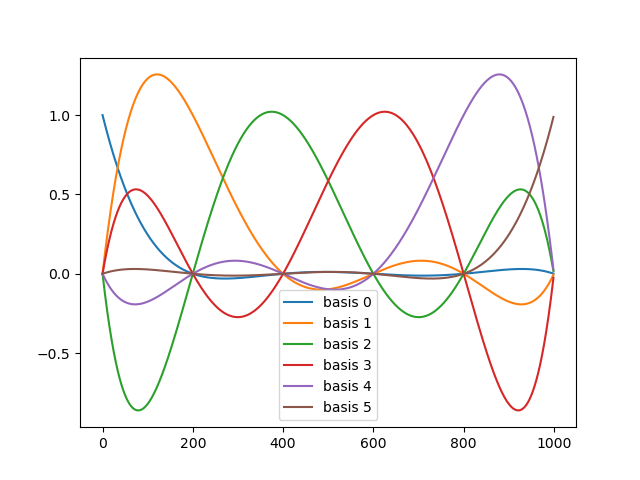
\includegraphics[width=0.75\textwidth]{chapters/element/plots/Lagrange5.png}
\caption{
The basis function of the Lagrange element of order 5. }
\label{fig:Lagrange5}
\end{center}
\end{figure}


The Hermite interpolation generalize the Lagrange interpolation by including also the first order derivative. 
The Hermite element is defined in terms of the Hermite interpolation. This is detailed in the following example. 

\begin{exmp}{\textbf{The Hermite element in 1D}.} 
\label{hermite:element}
Let us consider the Hermite interpolation onto $k+1$ points.  
Each point is associated with two degrees of freedom, the function evaluation and the evaluation of the first 
derivative of the function.  
using $m$ derivatives in each point. Hence,  
the number of degrees of freedom, or the number of equations defined by the specification of the nodal 
basis in Definition \ref{nodal:basis} are then $2(k+1)$. As such our polynomial space would be $\mathbb{P}_{2(k+1)}$.    
We may compute the nodal basis of the Hermite element: 
Let $H_j$ be the j'th nodal basis, expressed as  
\[ 
H_j = \sum_i \alpha_{ij} x^i 
\]
Then 
where $\alpha_{ij}$ are determined by 
\[ 
d_i(L_j) = L_j(x_i) = \delta_{ij} . 
\]
Here, lets split the degrees of freedom into even and odd numbers, where the even numbering refers to 
point evaluations whereas the odd numbers are the evaluation of the derivatives. 
That is 
\begin{align*} 
d_i(H_j) &= H_j(x_i)  &=  \delta_{ij}, \quad \mbox{ even } i,j   \\
d_i(H_j) &= H'_j(x) |_{x=x_i} &= \delta_{ij}, \quad \mbox{ odd } i,j  
\end{align*}

\end{exmp}


\section{Mapping a reference element onto a physical element. }

There are a two concepts that needs to be introduced before the above definition of the finite element is really useful.
The first concept is the mapping from a \emph{reference element} to a \emph{physical element}. 
A crucial observation is the fact that the mapping between an arbitrary cell of a general mesh and the reference cell can be generalized to 
a mapping between an arbitrary finite element on the mesh and a corresponding reference element.  
This observation is detailed below. 

Let $x$ and $\hat{x}$ be coordiates in the domains $T$ and $\hat{T}$, respectively. 
The domains $T$ and $\hat{T}$ are assumed of similar shape (isomorphic) 
and here we  
for simplicity assume an affine mapping between the coordinates:  
\[
x = F_T(\hat{x}) = A_T \hat{x} + x_0   
\]
The Jacobian of the mapping is 
\[
\frac{\partial x}{\partial \hat{x}} = J(\hat{x}) = A_T      
\]
For isoparametric elements, a basis function $\phi$
is the simply defined in terms of its associated function $\hat{\phi}$
on the reference
element, ie. 
\[
\phi(x) = \hat{\phi}(\hat{x}) .  
\]
With this definition we may easily evaluate integrals involving the basis functions: 
\[
\int_T \phi(x) \, dx = \int_{\hat{T}} \hat{\phi}(\hat{x}) \, det J \, d\hat{x},  
\]
where $det J$ is the determinant of $J$.  Furthermore, derivatives of the basis functions are readily available by using the chain-rule:  
\[
\frac{\partial \phi}{\partial x_i } = \sum_j  \frac{\partial \hat{\phi}}{\partial \hat{x}_j } \frac{\partial \hat{x}_j}{\partial \hat{x}_i } 
\]
As such the finite element engines may perform all the computations on the reference cells, which makes the implementation easy and efficient. 

\section{The connectivity of the mesh and the corresponding finite element space}

The second concept that needs to be dealt with is how to tie the finite elements together. 
Consider for example the Lagrange element of order 5 in 1D that was illustrated in Fig.~\ref{fig:Lagrange5}. We observe here that the basis function $0$ and $5$ are associated
with the edges $x=0$ and $x=1$, respectively. The other functions are all zero at the edges. Hence, the basis function $1, \ldots, 4$ do not connect 
to any other element, whereas the basis $0$ would directly connect to the a corresponding element on the left whereas basis $5$ connects to the 
an element on the right, if present. Hence the edge nodes defines the connectivity and hereby the continuity towards the neighbouring elements. 

The situation is more complicated in 2D and 3D. Consider the Lagrange element of order 1, 2, and 3 in Fig.~\ref{fig:lagrangeelement13}. Black, blue and red circles mark
the vertex, edge and interal nodes, which through the connectivity of the mesh defines the connectivity of the finite element filed. 
Consider the mesh in Fig.~\ref{fig:Lagrange8elements}. Clearly, the vertex node in the center, marked by a black circle is connected to all the 8 neighbouring elements. 
Hence, the corresponding basis function ties these eight elements together. On the other hand the edge degrees of freedom marked in 
blue only connect the two elements with common face. Finally, the internal degree of freedom does connect to any other elements and is often refered to as a bubble
function. 


\begin{figure}
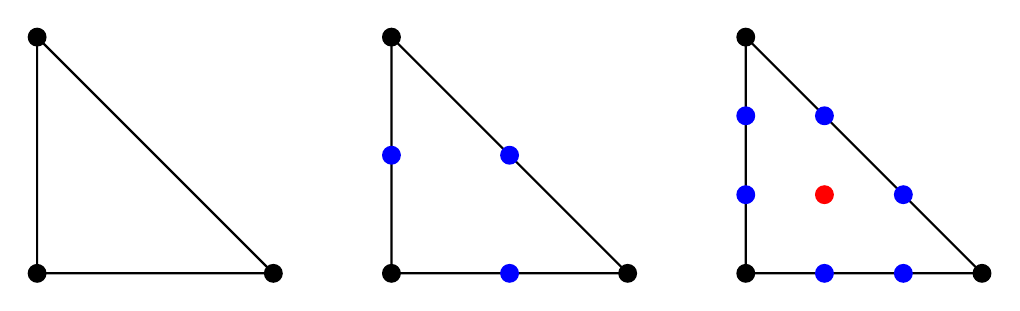
\begin{tikzpicture}[scale=3]

  % Define the vertices of the reference triangle
  \coordinate (A) at (0,0);
  \coordinate (B) at (1,0);
  \coordinate (C) at (0,1);

  \fill[black] (A) circle (0.04);
  \fill[black] (B) circle (0.04);
  \fill[black] (C) circle (0.04);



  % Draw the triangle
  \draw[thick] (A) -- (B) -- (C) -- cycle;
  % Add labels for clarity
%  \node[below left] at (A) {A};
%  \node[below right] at (B) {B};
%  \node[above left] at (C) {C};

  % done first triangle 

  % Define the vertices of the reference triangle
  \coordinate (A) at (1.5,0);
  \coordinate (B) at (2.5,0);
  \coordinate (C) at (1.5,1);

  % Draw the triangle
  \draw[thick] (A) -- (B) -- (C) -- cycle;

  % Define and draw the order 3 Lagrange nodes
  \coordinate (D) at (2.0,0);
  \coordinate (E) at (1.5,0.5);
  \coordinate (F) at (2.0,0.5);

  % Vertex nodes
  \fill[black] (A) circle (0.04);
  \fill[black] (B) circle (0.04);
  \fill[black] (C) circle (0.04);

  % Edge nodes
  \fill[blue] (D) circle (0.04);
  \fill[blue] (E) circle (0.04);
  \fill[blue] (F) circle (0.04);


  % Add labels for clarity
%  \node[below left] at (A) {A};
%  \node[below right] at (B) {B};
%  \node[above left] at (C) {C};

%  \node[below] at (D) {1/3};
%  \node[below] at (E) {2/3};
%  \node[right] at (F) {2/3};
%  \node[left] at (G) {1/3};

%  \node[above left] at (H) {1/3};
%  \node[above left] at (I) {2/3};

% Label the internal node
%  \node at (J) {(1/3, 1/3)};


  % Define the vertices of the reference triangle
  \coordinate (A) at (3,0);
  \coordinate (B) at (4,0);
  \coordinate (C) at (3,1);

  % Draw the triangle
  \draw[thick] (A) -- (B) -- (C) -- cycle;

  % Define and draw the order 3 Lagrange nodes
  \coordinate (D) at (3.333,0);
  \coordinate (E) at (3.667,0);
  \coordinate (F) at (3.667,0.333);
  \coordinate (G) at (3.333,0.667);
  
  \coordinate (H) at (3,0.333);
  \coordinate (I) at (3,0.667);
  \coordinate (J) at (3.333,0.333);

  % Vertex nodes
  \fill[black] (A) circle (0.04);
  \fill[black] (B) circle (0.04);
  \fill[black] (C) circle (0.04);

  % Edge nodes
  \fill[blue] (D) circle (0.04);
  \fill[blue] (E) circle (0.04);
  \fill[blue] (H) circle (0.04);
  \fill[blue] (I) circle (0.04);
  \fill[blue] (F) circle (0.04);
  \fill[blue] (G) circle (0.04);

  % Internal node
  \fill[red] (J) circle (0.04);

  % Add labels for clarity
%  \node[below left] at (A) {A};
%  \node[below right] at (B) {B};
%  \node[above left] at (C) {C};

%  \node[below] at (D) {1/3};
%  \node[below] at (E) {2/3};
%  \node[right] at (F) {2/3};
%  \node[left] at (G) {1/3};

%  \node[above left] at (H) {1/3};
%  \node[above left] at (I) {2/3};

% Label the internal node
%  \node at (J) {(1/3, 1/3)};

\end{tikzpicture}
\label{fig:lagrangeelement13}
\caption{The Lagrange element of order 1, 2, 3 on the reference triangle in 2D. Black circles mark the vertex nodes, blue the edge nodes and red the internal nodes. }
\end{figure}



\begin{figure}
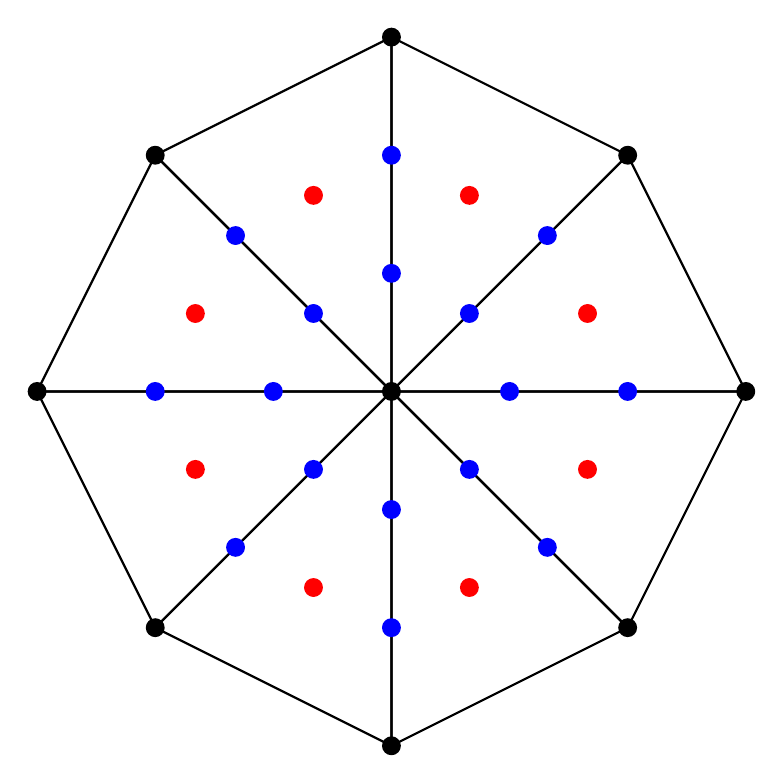
\begin{tikzpicture}[scale=3]
\draw[black, thick] (0,0) -- (1,1) -- (0,1.5) -- cycle;
\draw[black, thick] (0,0) -- (1,1) -- (1.5,0) -- cycle;
\draw[black, thick] (0,0) -- (1,-1) -- (1.5,0) -- cycle;
\draw[black, thick] (0,0) -- (1,-1) -- (0,-1.5) -- cycle;
\draw[black, thick] (0,0) -- (-1,-1) -- (-1.5,0) -- cycle;
\draw[black, thick] (0,0) -- (-1,-1) -- (0,-1.5) -- cycle;
\draw[black, thick] (0,0) -- (-1,1) -- (0,1.5) -- cycle;
\draw[black, thick] (0,0) -- (-1,1) -- (-1.5,0) -- cycle;

\coordinate (A1) at (0,0);
\coordinate (A2) at (1.5,0);
\coordinate (A3) at (-1.5,0);
\coordinate (A4) at (0,1.5);
\coordinate (A5) at (0,-1.5);
\coordinate (A6) at (1,1);
\coordinate (A7) at (1,-1);
\coordinate (A8) at (-1,1);
\coordinate (A9) at (-1,-1);




\coordinate (B1) at (0,0.5);
\coordinate (B2) at (0,1);
\coordinate (B3) at (0,-0.5);
\coordinate (B4) at (0,-1);
\coordinate (B5) at (0.5,0);
\coordinate (B6) at (1,0);
\coordinate (B7) at (-0.5,0);
\coordinate (B8) at (-1,0);
\coordinate (B9) at (0.33,0.33);
\coordinate (B10) at (0.66,0.66);
\coordinate (B11) at (-0.33,-0.33);
\coordinate (B12) at (-0.66,-0.66);
\coordinate (B13) at (0.33,-0.33);
\coordinate (B14) at (0.66,-0.66);
\coordinate (B15) at (-0.33,0.33);
\coordinate (B16) at (-0.66,0.66);

\coordinate (C1) at (0.33,0.83);
\coordinate (C2) at (-0.33,0.83);
\coordinate (C3) at (-0.33,-0.83);
\coordinate (C4) at (0.33,-0.83);
\coordinate (C5) at (0.83,0.33);
\coordinate (C6) at (-0.83,0.33);
\coordinate (C7) at (-0.83,-0.33);
\coordinate (C8) at (0.83,-0.33);

\fill[black] (A1) circle (0.04);
\fill[black] (A2) circle (0.04);
\fill[black] (A3) circle (0.04);
\fill[black] (A4) circle (0.04);
\fill[black] (A5) circle (0.04);
\fill[black] (A6) circle (0.04);
\fill[black] (A7) circle (0.04);
\fill[black] (A8) circle (0.04);
\fill[black] (A9) circle (0.04);
\fill[blue] (B1) circle (0.04);
\fill[blue] (B2) circle (0.04);
\fill[blue] (B3) circle (0.04);
\fill[blue] (B4) circle (0.04);
\fill[blue] (B5) circle (0.04);
\fill[blue] (B6) circle (0.04);
\fill[blue] (B7) circle (0.04);
\fill[blue] (B8) circle (0.04);
\fill[blue] (B9) circle (0.04);
\fill[blue] (B10) circle (0.04);
\fill[blue] (B11) circle (0.04);
\fill[blue] (B12) circle (0.04);
\fill[blue] (B13) circle (0.04);
\fill[blue] (B14) circle (0.04);
\fill[blue] (B15) circle (0.04);
\fill[blue] (B16) circle (0.04);
\fill[red] (C1) circle (0.04);
\fill[red] (C2) circle (0.04);
\fill[red] (C3) circle (0.04);
\fill[red] (C4) circle (0.04);
\fill[red] (C5) circle (0.04);
\fill[red] (C6) circle (0.04);
\fill[red] (C7) circle (0.04);
\fill[red] (C8) circle (0.04);



%\node[below left] at (A) {A};
%\node[below left] at (B) {B};
\end{tikzpicture}
\label{fig:Lagrange8elements}
\caption{A simple mesh with 8 triangles all meeting at a common point. 
Here, we have marked (only) three nodes associated with a third order Lagrange element: A vertex node (black), an edge node(blue) and an internal node (red).  
Marking all nodes would yield 9 vertex nodes,  16 edge nodes, and 8 internal nodes.  }
\end{figure}



\kent{Describe also briefly CR, RT, Nedelec, MTW elements}



\begin{figure}
\begin{center}
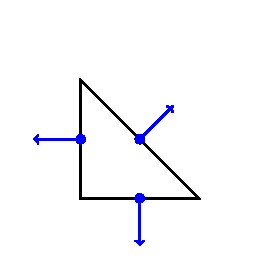
\includegraphics[width=5cm]{chapters/element/rt.pdf}
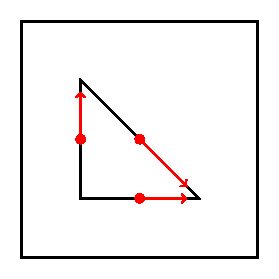
\includegraphics[width=5cm]{chapters/element/nedlec.pdf}
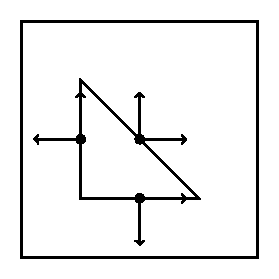
\includegraphics[width=5cm]{chapters/element/cr.pdf}
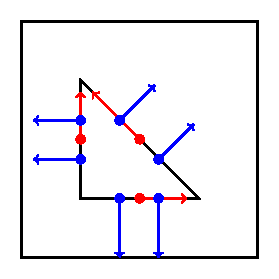
\includegraphics[width=5cm]{chapters/element/mtw.pdf}
	\caption{Illustration of the Raviart-Thomas element (upper left), the  Nedelec element (upper right), the Crouizeix-Raviart element (lower left), and the Mardal-Tai-Winther (lower right), all of the lowest order possible. 
Face normal vectors are colored in blue, whereas face tangents are colored in red. Black arrows are  
align with the underlying coordinate system. 
} \label{fig:rtetc}
\end{center}

\end{figure}

\section{Approximation in different function spaces, $L^2$, $H^1$, $H^2$, $H(\mbox{div})$, and $H(\mbox{curl})$ }

The function spaces 
$L^2$, $H^1$, $H^2$, $H(\mbox{div})$, and $H(\mbox{curl})$ 
have different requirement with respect to continuity across cell boundaries (within a cell, all common finite elements are 
polynomials and hence $C^\infty$). In $L^2$ no continuity is required and as such there is no need to tie vertex or face
degrees of freedom together. Hence, for example, in Fig. \ref{fig:dgcg} we have a mesh in 1D consisting of two cells $(0, 0.5)$ and
$(0.5, 1.0)$. Locally, the first order Lagrange element is defined in terms of the vertices, ie. for the first element the points
$x=0.0$ and $x=0.5$ whereas for the second element the points are $x=0.5$ and $x=1.0$. Both a discontinuous and a continuous
function is shown in Fig. \ref{fig:dgcg}, corresponding to discontinuous and continuous Lagrange elements on this simple mesh. 
A crucial difference between them is whether the function is continuous at $x=0.5$ or not. 


\begin{figure}
\begin{center}
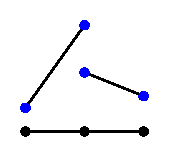
\includegraphics[width=5cm]{chapters/element/dg.pdf}
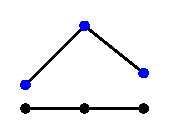
\includegraphics[width=5cm]{chapters/element/cg.pdf}
\caption{Piecewise discontinuous and continuous first order polynomials defined in terms of two cells in 1D. }  
\label{fig:dgcg}
\end{center}
\end{figure}



\section{Exercises}


\begin{exercise}
Consider two triangles $T_0$ and $T_1$ defined by the vertices $(0,0), (1,0), (1,0)$ and
$(3,4), (4,2), (4,4)$. Computing the mapping between them.  
\end{exercise}


\begin{exercise}
\label{hermite:interval}
Make a Python code that defines a Hermite on the unit interval.       
\end{exercise}



\begin{exercise}
\label{lagrange:triangle}
Make a Python code that defines a Lagrange element of arbitrary order on the reference triangle 
consisting of the vertices $(0,0)$, $(1,0)$ and $(0,1)$. Let $\mathbb{P}_k = \{ x^i y^j \} \mbox{ for } i,j \mbox{ such that } i+j \le k\} $     
\end{exercise}

\begin{exercise}
Check that the interpolation result
of the Bramble-Hilbert lemma \ref{bramblehilbert} applies to the Lagrange interpolation on the unit line. Consider 
for example a function $f = sin(x)$ on the unit interval. The function $f$ is a good example as it cannot be expressed 
as a polynomial of finite order, but can be approximated arbitrary well. 
\end{exercise}

\begin{exercise}
Compute the condition number of the mass matrix when using the Lagrange and the Hermite basis. Compare it with the condition
number when using the basis consisting of monomials, ie. $(1, x, x^2, \ldots)$.   
	The mass matrix on the unit interval  is the matrix $M_{ij} = \int_0^1 \phi_i \phi_j \, dx $ where $\{\phi_i\}$ is 
	the set of basis functions in use. 
\end{exercise}





